\section{电流强度跟电压的关系}\label{sec:8-5}

我们知道,导体中的电流是由电压产生的,那么,电流强度跟电压的大小又有什么关系呢?
人们会自然地想到:在同一电路上,电压越大,电流强度就越大。实际上也的确是这样。
用一节干电池来点亮手电筒小灯泡,小灯泡不怎么亮;用两节干电池,小灯泡就亮起来了。
这说明加在小灯泡上的电压越大,通过小灯泡的电流越强。下面我们用实验进一步研究电流强度跟电压的关系。

\begin{figure}[htbp]
    \centering
    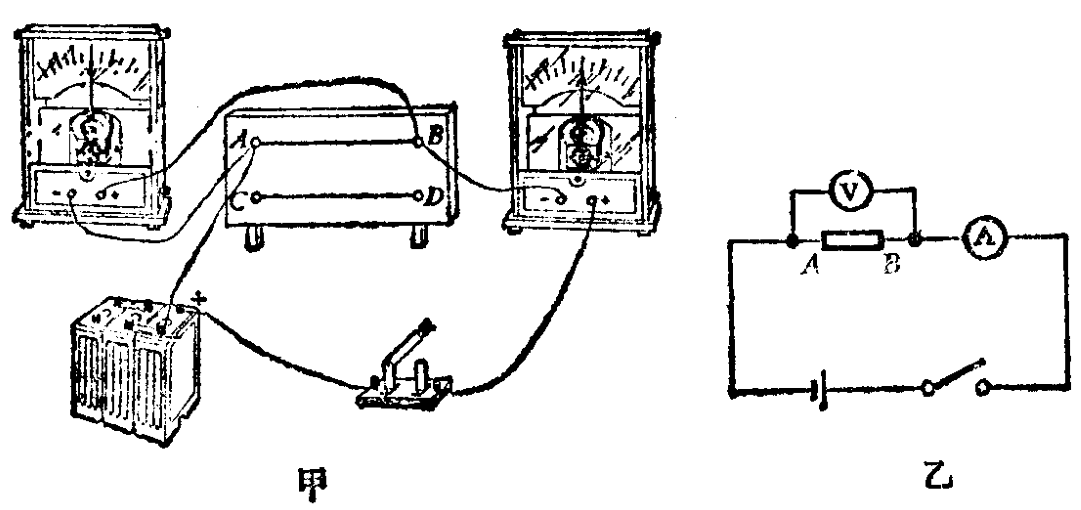
\includegraphics[width=0.7\textwidth]{../pic/czwl2-ch8-16}
    \caption{}\label{fig:8-16}
\end{figure}

图 \ref{fig:8-16} 甲表示我们所用的实验装置,立着的木板上张着 $AB$、$CD$ 两条不同的导线。
先用导线 $AB$ 做实验,照图 \ref{fig:8-16} 乙连接电路。
用改变串联的电池数目的办来改变导线 $AB$ 两端的电压,由伏特表读出这个电压值,
由安培表读出导线中的电流。表 \ref{tab:8-1} 记录了测得的数据。

\begin{table}[htbp]
    \centering
    \caption{用导线 $AB$ 实验时的记录}\label{tab:8-1}
    \begin{tblr}{
        hlines, vlines,
        colspec={cccc},
        column{2-4} = {wd=4em},
    }
        电压(伏特) & 2 & 4 & 6 \\
        电流强度(安培)& 0.4 & 0.8 & 1.2
    \end{tblr}
\end{table}

从测得的数据可以看出,导线 $AB$ 两端的电压增大到几倍,其中的电流强度也增大到几倍。
导线 $AB$ 中的电梳强度跟它两端的电压成正比。

现在换用导线 $CD$ 做实验,并把测得的数据列在表 \ref{tab:8-2} 中。
我们看到,虽然在相同的电压下,通过导线 $CD$ 的电流跟通过导线 $AB$ 的电流不同,
但是导线 $CD$ 中的电流强度仍然跟它两端的电压成正比。

\begin{table}[htbp]
    \centering
    \caption{用导线 $CD$ 实验时的记录}\label{tab:8-2}
    \begin{tblr}{
        hlines, vlines,
        colspec={cccc},
        column{2-4} = {wd=4em},
    }
        电压(伏特) & 2 & 4 & 6 \\
        电流强度(安培)& 0.2 & 0.4 & 0.6
    \end{tblr}
\end{table}


再换用其他导线做实验,都会得到上述正比关系。这样,我们得到结论:

\CJKunderwave{导体中的电流强度跟这段导体两端的电压成正比}。

